\documentclass[border=10pt]{standalone}
\usepackage{pgfplots}
\pgfplotsset{compat=1.18, trig format plots=rad}
\begin{document}
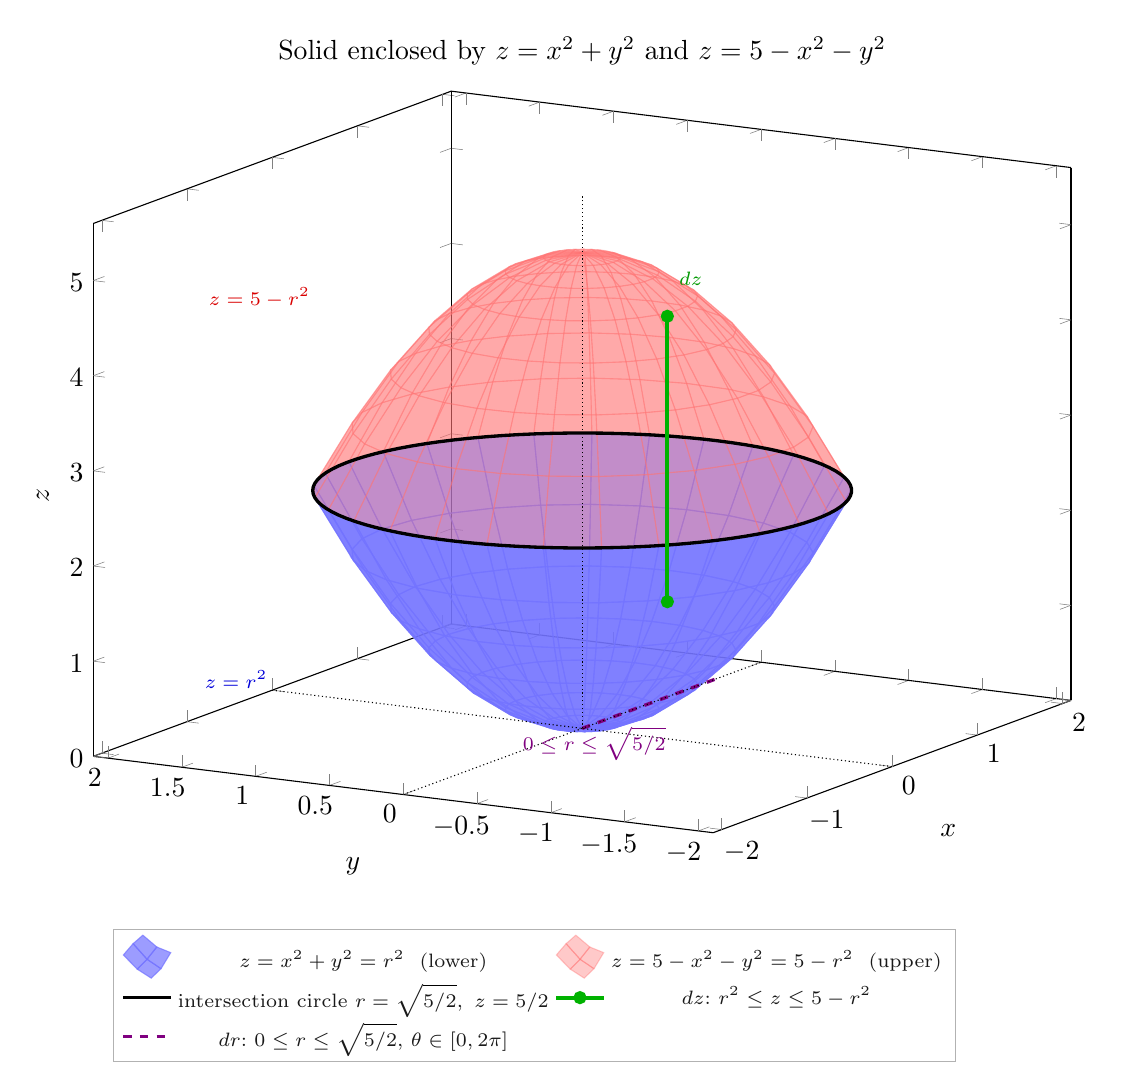
\begin{tikzpicture}
\begin{axis}[
    width=14cm, height=11cm,
    view={-60}{16},
    xmin=-2.1, xmax=2.1, ymin=-2.1, ymax=2.1, zmin=0, zmax=5.6,
    xlabel={$x$}, ylabel={$y$}, zlabel={$z$},
    axis background/.style={white},
    enlargelimits=false,
    legend style={at={(0.02,-0.13)}, anchor=north west, font=\scriptsize,
                  draw=black!30, fill=white, fill opacity=0.9, legend columns=2},
    title={Solid enclosed by $z=x^2+y^2$ and $z=5-x^2-y^2$},
]
% ---- lower paraboloid  z = r^2  over the disk r <= sqrt(5/2) ----
\addplot3[surf, shader=flat, blue!55, opacity=0.70,
          domain=0:6.2832, samples=30, samples y=8, y domain=0:1.5811]
  ({y*sin(x)}, {y*cos(x)}, {y^2});
\addlegendentry{$z=x^2+y^2=r^2$ \ (lower)}
% ---- upper paraboloid  z = 5 - r^2  over the same disk ----
\addplot3[surf, shader=flat, red!55, opacity=0.38,
          domain=0:6.2832, samples=30, samples y=8, y domain=0:1.5811]
  ({y*sin(x)}, {y*cos(x)}, {5-y^2});
\addlegendentry{$z=5-x^2-y^2=5-r^2$ \ (upper)}
% ---- circle of intersection ----
\addplot3[very thick, black, domain=0:6.2832, samples=100, samples y=0]
  ({1.5811*cos(x)}, {1.5811*sin(x)}, {2.5});
\addlegendentry{intersection circle $r=\sqrt{5/2},\ z=5/2$}
% ---- vertical element (direction of dz) at r = 1 ----
\addplot3[green!70!black, line width=1.5pt, mark=*,
          mark options={fill=green!70!black, scale=0.8}]
  coordinates {(1,0,1) (1,0,4)};
\addlegendentry{$dz$:\ $r^2\le z\le 5-r^2$}
% ---- radial element (direction of dr) ----
\addplot3[violet, dashed, line width=1.2pt] coordinates {(0,0,0) (1.5811,0,0)};
\addlegendentry{$dr$:\ $0\le r\le\sqrt{5/2}$,\ $\theta\in[0,2\pi]$}
% ---- coordinate axis hints ----
\addplot3[black, densely dotted, thin] coordinates {(-2.1,0,0) (2.1,0,0)};
\addplot3[black, densely dotted, thin] coordinates {(0,-2.1,0) (0,2.1,0)};
\addplot3[black, densely dotted, thin] coordinates {(0,0,0) (0,0,5.6)};
\node[blue!85!black] at (axis cs:-1.55,1.45,0.75) {\scriptsize $z=r^2$};
\node[red!85!black] at (axis cs:-1.45,1.35,4.75) {\scriptsize $z=5-r^2$};
\node[green!60!black] at (axis cs:1.62,0.2,4.15) {\scriptsize $dz$};
\node[violet] at (axis cs:0.8,0.38,-0.5) {\scriptsize $0\le r\le\sqrt{5/2}$};
\end{axis}
\end{tikzpicture}
\end{document}
